\documentclass{amia}
\usepackage{graphicx}
\usepackage[labelfont=bf]{caption}
\usepackage[superscript,nomove]{cite}
\usepackage{color}


\begin{document}


\title{Title of Your Submission}

\author{Firstname A. Lastname, Degrees$^{1}$, Firstname B. Lastname, Degrees$^{2}$}

\institutes{
    $^1$Institution, City, State, Country (if applicable); $^2$Institution, City, State, Country (if applicable)\\
}

\maketitle

\noindent{\bf Abstract}

\textit{Abstract text goes here, justified and in italics.  The abstract would normally be one paragraph long.  See Table 1. for appropriate abstract length by submission type.}

\section{Introduction}

This is where you introduce your topic providing examples. And then give a brief overview to the reader of what they should expect while reading your review.

\section{Current Literature} %please rename this

For the main body of your review, you should organize the literature according to common themes

For this think about: 
\begin{itemize}
    \item what algorithms have people used
    \item how did they represent their data
    \item what pre-processing did they do to their data
    \item what post-processing did they do to their data
    \item what datasets did they use
    \item how did they evaluate their proposed systems
    \begin{itemize}
        \item what methodology did they use (train/test split versus k-fold crossvalidation
        \end{itemize}
\end{itemize}

These can be included in subsections of the Main Body. See an example of subsections below.

\section{Compare and Contrast}

Here is where you can compare and contrast those literatures. Please, include a table; remember to reference and describe the table. 

\section{This section contains examples}

This sentence has two reference citations\cite{leaman2008banner, yarowsky1995unsupervised}.

This sentence has one reference citation\cite{bort2020discovery}.

\subsection{Here is a subsection}
    Here is an example subsection

\section{Back to another section with examples}

More text of an additional paragraph, with a figure reference (Figure ~\ref{fig1}) and a figure inside a Word text box below.  Figures need to be placed as close to the corresponding text as possible and not extend beyond one page.\\
\begin{figure}[h!]
\centering
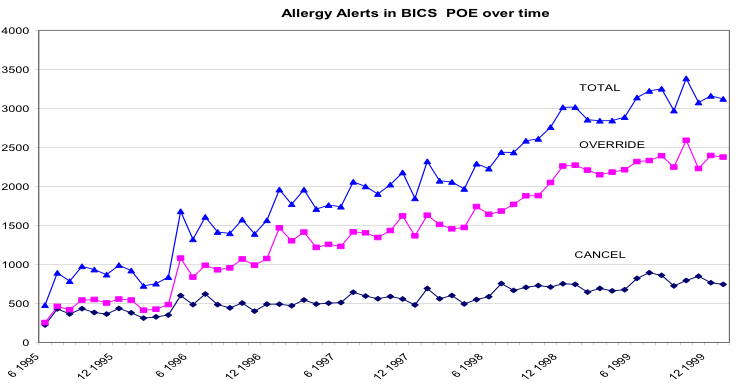
\includegraphics[scale=1]{pics/figure1.png}
\caption{Total allergy alerts, overridden alerts, or drug order cancelled.}
\label{fig1}
\end{figure}

This is additional text added just to show the one-column formatting.  This is additional text added just to show the one-column formatting.  This is additional text added just to show the one-column formatting.  This is additional text added just to show the one-column formatting.  This is additional text added just to show the one-column formatting.  This is additional text added just to show the one-column formatting.  This is additional text added just to show the one-column formatting.

This paragraph contains a reference to a table just below (Table 1).  All tables need to be placed as close to the corresponding text as possible, But each individual table should be on one page and not extend to multiple pages unless labeled as ``��Continued"��.

\begin{table}[h]
\centering
\caption{Submission type, abstract length, and page length maximum for AMIA submissions.}
  \begin{tabular}{|l|l|l|}
  \hline
    \textbf{Submission Type}    & \textbf{Abstract Length}  & \textbf{Page Length Maximum**} \\ \hline
    Paper  & 125-150 words  & Ten   \\ \hline
    Student Paper  & 125-150 words  & Ten \\ \hline
    Poster  &50-75 words*   & One \\ \hline
    Podium  Abstract & 50-75 words*  & Two \\ \hline
    Panel   &150-200 words  & Three \\ \hline
    System Demonstrations    &150-200 words  & One \\ \hline
  \end{tabular}
\end{table}


This is another paragraph.

\section{Conclusion}

The conclusion should:
\begin{itemize}
    \item summarize the important aspects of the existing body of literature;
    \item evaluate the current state of the literature reviewed;
    \item identify significant flaws or gaps in existing knowledge;
    \item outline areas for future study;
    \item link your research to existing knowledge
\end{itemize}

\makeatletter
\renewcommand{\@biblabel}[1]{\hfill #1.}
\makeatother



\bibliographystyle{unsrt}
\bibliography{refs}

\end{document}

